\documentclass[manuscript=cmatex]{achemso}
\usepackage[usenames,dvipsnames]{xcolor}
% \definecolor{linkcolor}{RGB}{0,0,240}
\usepackage{achemso}
\usepackage{makecell}
\usepackage{xr-hyper}
\usepackage{hyperref}
\usepackage{hypcap}
\usepackage{appendix}
\usepackage{upgreek}
\usepackage{chemmacros}
\usepackage{siunitx}
\usepackage{textcomp}
\usepackage{natmove}

\captionsetup{font={rm,small}}
\SectionNumbersOn
\usechemmodule{reactions}
\chemsetup{modules=reactions}

\usepackage[USenglish]{babel}
\addto\captionsenglish{\renewcommand\chaptername{Section}}
\usepackage{graphicx,array,tabularx,mathtools,siunitx,amsmath,multirow,longtable,float}
\usepackage[nameinlink,noabbrev,capitalize]{cleveref}
\setlength{\footskip}{0.25in}
\usepackage[labelformat=simple]{subfig}
\graphicspath{ {./imgs/} }
%\usepackage[version=4]{mhchem}
\usepackage{cleveref}
\usepackage[labelfont=bf]{caption}
\hypersetup{
  pdfstartview = {XYZ},
  allcolors = linkcolor,
  bookmarksopen,
  bookmarksnumbered,
  colorlinks=false,
  filecolor=black,
  citecolor = black,      
  urlcolor=black,
}

%%%%%%%%%%%%%%%%%%%%%%%%%%%%%%%%%%%%%%%% 
%%%%%%%%%%% 
% \numberwithin{reaction}{section}

\makeatletter
\@ifundefined{ignorespacesafterend}{\def\ignorespacesafterend{\global\@ignoretrue}}{}
\newenvironment{subreactions}{%
  \refstepcounter{reaction}%
  \protected@edef\theparentequation{\thereaction}%
  \setcounter{parentequation}{\value{reaction}}%
  \setcounter{reaction}{0}%
  \def\thereaction{\theparentequation\alph{reaction}}%
  \ignorespaces
}{%
  \setcounter{reaction}{\value{parentequation}}%
  \ignorespacesafterend
}

\makeatother
\title          {Evolution of Copper Surfaces under Plasma Oxidation: Molecular Dynamics Study with Neural Network Potentials}
\author         {Yantao Xia}
\affiliation    {Department of Chemical and Biomolecular Engineering, University of California, Los Angeles, CA 90095, USA}
\email          {xyttyxy@ucla.edu}
\author         {Philippe Sautet}
\affiliation    {Department of Chemical and Biomolecular Engineering, University of California, Los Angeles, CA 90095, USA}
\alsoaffiliation    {Department of Chemistry and Biochemistry, University of California, Los Angeles, CA 90095, USA}
\email          {sautet@ucla.edu}

\makeatletter
\def\@maketitle{%
  \newpage
  \null
  \vskip 2em%
  \begin{center}%
  \let \footnote \thanks
    {\LARGE \@title \par}%
    \vskip 1em%
    {\Large Supplementary Information\par}%
    \vskip 1.5em%
    {\large
      \lineskip .5em%
      \begin{tabular}[t]{c}%
        \@author
      \end{tabular}\par}%
    \vskip 1em%
  \end{center}%
  \par
  \vskip 1.5em}
\makeatother

%%%%%%%%%%%%%%%%%%%%%%%%%%%%%%%%%%%%%%%%%%%%%%%%%%% 
% table formatting commands
\renewcommand{\thesubfigure}{\relax} % no labels on subfigures
\begin{document}
\maketitle
\section{Additional Computational Details}
\subsection{Choice of the exchange-correlation functional}
We estimated the number of required structures to determine whether hybrid functions (e.g. HSE03) is feasible following the ``active learning'' method proposed in \textbf{CITE}. Figure \textbf{REF} shows that at \textit{NUM} structures, the training set error cannot be decreased to a satisfactory value. Based on this it was concluded that hybrids functionals are too expensive for this application. We also note in passing that the exchange-correlation functional must describe properties of both the metal, the molecular and atomic modifier, and the oxide phases accurately. While hybrids could improve the description of the correlated oxide, they in general do not describe the metals well. Hence, the versatile PBE functional is used.
\subsection{Neural network architecture}
% 
% Additional computational details regarding the architecture of the neural network and the setup of the MD simulations are given in the \textbf{supplementary information}
\subsection{Details regarding data cleaning}
% It was found, later during training, that data cleaning is crucial to the success of training. The cleaning process removes configurations with extremely short bond lengths. These configurations create electronic convergence problems during subsequent DFT calculations. Even when DFT is successful, their energies and forces end up as outliers during training. Hence, a simple cleaning procedure ensures the minimum \ch{Cu}-\ch{O} and \ch{Cu}-\ch{Cu} bond distances are above predetermined threshold values.
% Data cleaning is done before and after DFT calculations, based on geometric and energetic criteria, respectively (see \textbf{SI}). It was discovered that the short bond distance interaction was not described well under this parametrization, leading to unstabilities during high energy ion impact simulations. As a result, the inner wall repulsion term, implemented in ReaxFF, was re-parametrized to the potential energy curves of \ch{Cu}-\ch{Cu}, \ch{Cu}-\ch{O}, and \ch{O}-\ch{O} dimers.
\subsection{Additional training and model validation information}
\begin{figure}[h]
  \centering
  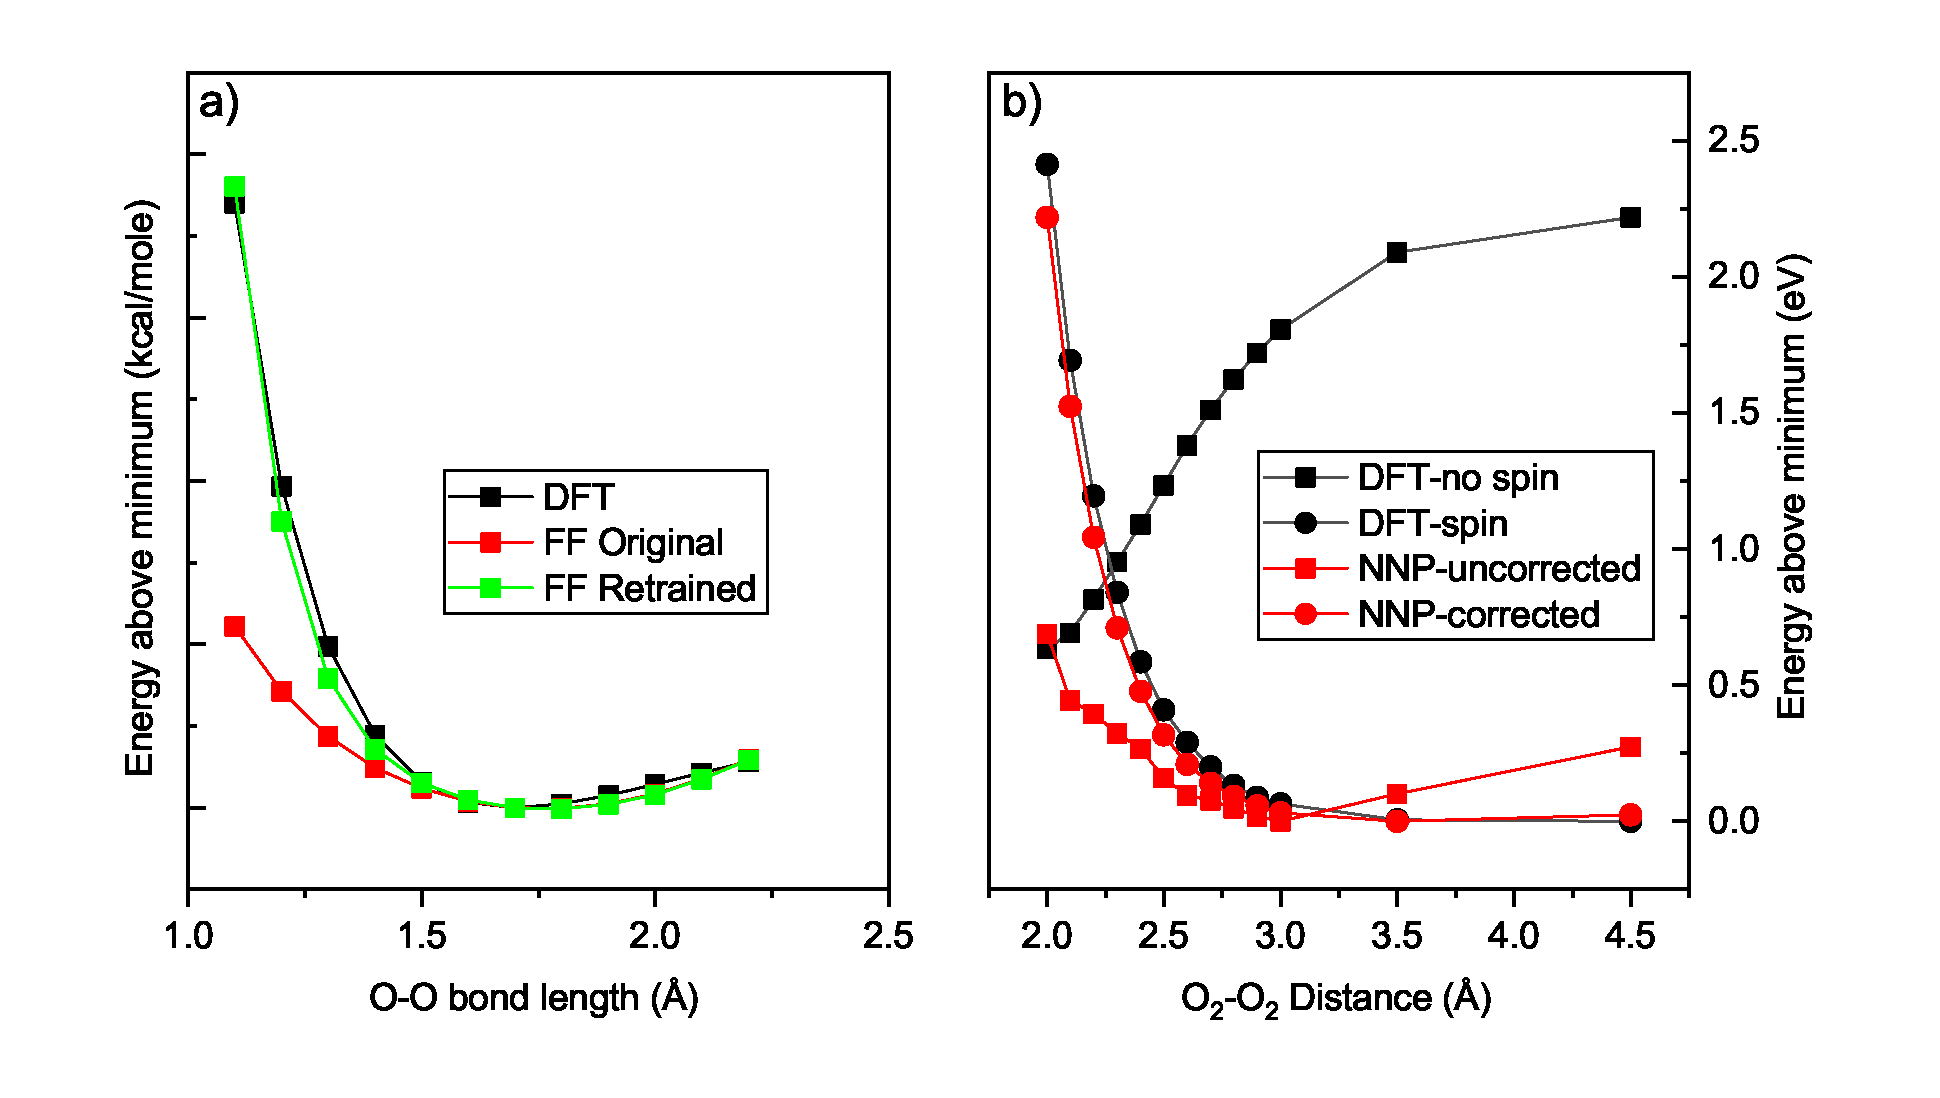
\includegraphics[width=\textwidth]{o2o4}
  \caption[PES of \ch{O2}-\ch{O2} interaction using DFT and NNP]{\textbf{(a)}: comparison of potential energy of an \ch{O2} molecule using literature ReaxFF parameter set (FF original), reparametrized ReaxFF parameter set (FF-retrained), and DFT. \textbf{(b)}: comparison of the potential energy surface two shoulder-to-shoulder \ch{O2} molecules, using spin unpolarized DFT(DFT-no spin), spin polarized DFT (DFT-spin), and two parameter sets of the neural network potential before and after correcting for oxygen clustering.}
  \label{fig:o4}
\end{figure}

% The comparison of the curves before and after the re-parametrization can be seen in \textbf{SI}.
% A script (see SI) was created to automatically detect impact events and select snapshots centered around them.

% The training routines were able to minimize the energy and force errors on the test set to \SI{2.32}{meV / atom} and $\SI{0.15}{eV/\angstrom}$, respectively. The new neural network parametrization, termed \textbf{nnp1}, was used in identical MD impact simulations as those used to generate \textbf{md0}, to generate a new set of snapshots. In subsequent steps, the ReaxFF force field itself, and the ReaxFF-based \textbf{md0} dataset, were not used. Again, 25 distinct MD runs were performed. After a cleaning procedure identical to that applied to \textbf{md0}, yielding \textbf{md1} dataset, containing 2716 structures. Before training was performed on this new dataset, the self-consistency of the neural network potential \textbf{nnp1} was tested by calculating its prediction error on the dataset obtained via MD driven by itself (\textbf{md1}), as an benchmark for the out-of-sample error. Not surprisingly, the energy error is \SI{88.67}{meV / atom} and the force error is $\SI{1.98}{eV/\angstrom}$. The fact that the out-of-sample error is almost two orders of magnitude higher than the in-sample error is used as an indication that the sample (ReaxFF-generated at this stage) has a different underlying ``distritbuion'' than the ground truth (in this case, the DFT potential energy surface), in accordance with statistical learning theory. Therefore, the neural network potential is retrained on the dataset composed of \textbf{md1}, to yield a test set error \SI{3.14}{meV / atom} and $\SI{0.17}{eV/\angstrom}$, respectively on energies and forces. New MD structures were generated (\textbf{md2}), and again the out-of-sample prediction error is calculated to be \SI{2.78}{meV / atom} and $\SI{0.13}{eV/\angstrom}$, respectively. This indicates that the neural network potential, within the MD setup used to generate the training configurations, does not extrapolate. As a finishing step, \textbf{md1} and \textbf{md2} are combined to retrain the neural network potential, yielding \textbf{nnp2}. 

% The \textbf{nnp2} potential, however, was only trained on a $(3\times3)$ Cu (100) cell with 5 layers. To avoid artifacts introduced by periodic boundary conditions, the production simulations needs to be run on much larger cells. Attempting to do so, however, creates extrapolation problem. Two reasons are underlying. The first is that in the small cell used for training, the lateral dimensions were shorter than the cutoff length of the neural network potential. When the oxygen molecule dissociates, the individual atoms is always inside the cutoff spheres of each other, preventing the chemical environment of isolated oxygen atom on the copper slab from being included in the training set. The second reason is the thickness of the slab is less than twice the cutoff radius. Therefore, even the central \ch{Cu} atom is not completely surrounded by other \ch{Cu} atoms, preventing the bulk copper environment from being described accurately. A parallel problem of not able to describe bulk oxide manifests itself when the oxide thickness approaches $2r_c$. As the choice of a $(3\times3\times5)$ slab model was to keep the cost of dataset preparation low, these problems were remedied by supplementary datasets of 1) single O atom impact simulations, concentrated on describing the very first impacting event (\textbf{impact\_initial}, 604 configurations), 2) thick $(3\times3\times8)$ \ch{Cu} and oxide slabs, produced by running impact simulations at elevated temperatures until the entire slab is oxidized (\textbf{thick}, 256 configurations). 3) snapshots of high temperature equilibrium MD of bulk \ch{CuO} and \ch{Cu2O} supercells (\textbf{bulk}, 300 configurations). After these supplemental configurations were added to the dataset, the retrained NNP was able to sustain simulations upto 1 nanosecond on a $(20\times20\times10)$ slab with 4000 atoms. Simulations on larger slabs are feasible but not attempted.
% The structures are illustrated in \textbf{SI}
% The details of characterizing this thickness from the MD trajectory is given in \textbf{SI}.
% since the deposition rate is much higher than what is likely under the experimental pressures (see comparison in \textbf{SI})
% and the implemented collision event tracking method (see \textbf{SI}).
% The $q_6$ parameters of \ch{Cu} and \ch{O} overlap each other and can be found in the \textbf{SI}.
% To study the thermal activation of diffusion inside the oxide, the diffusivities at various temperatures are calculated (see details in \textbf{SI}).
%\clearpage
%\bibliography{ref}

\end{document}
